\chapter{佐佐木希案例分析与模板要素展示}

本章以佐佐木希的公开职业经历为线索，同时用图表、图片与表格展示 `thesis-nju-master` 的常见排版
组件。这里的插图和表格主要承担“演示模板能力”的角色，因此强调的是页面结构、题注样式和版面
组织方式，而不是构建严格的经验研究数据库。

\section{职业阶段映射示例}

职业转型的第一步，是把零散的曝光事件组织为阶段化路径。对于佐佐木希而言，模特时期提供了初始
识别度，影视与综艺时期扩大了受众覆盖面，争议事件带来了叙事断裂，而社交平台经营则成为重启阶段
的关键抓手。图~\ref{fig:nju-stage-map} 用流程图形式展示这一阶段映射。

\begin{figure}[H]
  \centering
  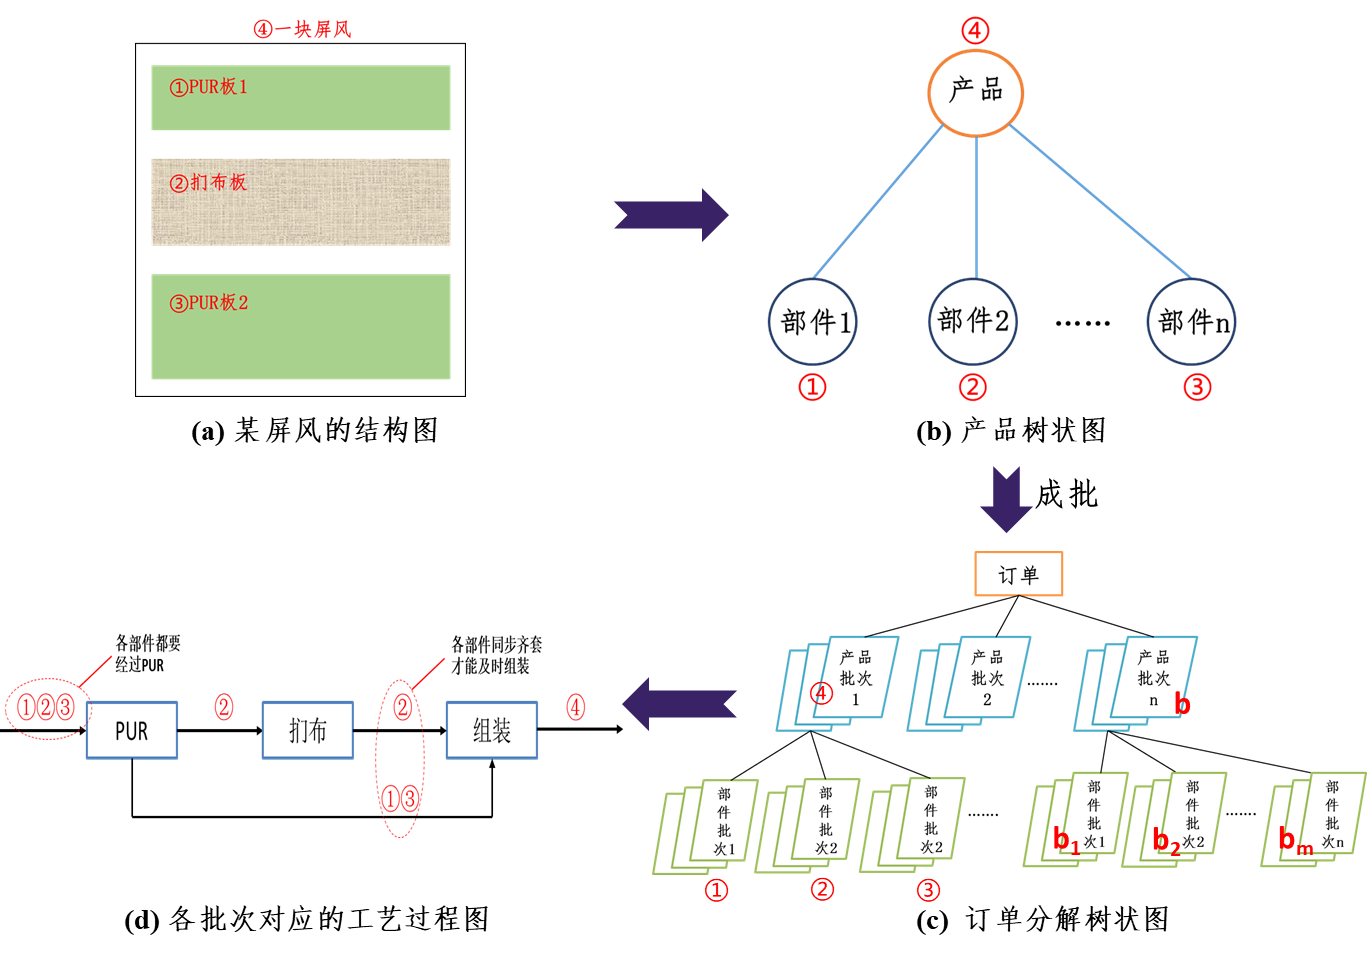
\includegraphics[width=0.8\textwidth]{assets/demo/figure-process-map.png}
  \caption{佐佐木希跨媒介职业路径的阶段映射示意}
  \label{fig:nju-stage-map}
\end{figure}

\section{曝光节奏变化示例}

如果把职业转型理解为内容运营项目，那么仅有“出现在哪个平台”是不够的，还需要观察“以什么节奏
持续出现”。危机后的重启阶段，往往不是靠一次高强度曝光完成，而是依赖频率更稳定、语气更日常的
内容供给。图~\ref{fig:nju-exposure-trend} 以曲线图示意不同阶段的曝光节奏变化，用来展示图题、编号
与正文之间的空间关系。

\begin{figure}[H]
  \centering
  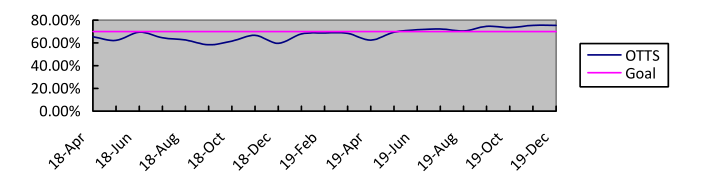
\includegraphics[width=0.72\textwidth]{assets/demo/figure-otd-chart.png}
  \caption{不同阶段公开曝光节奏的示意变化}
  \label{fig:nju-exposure-trend}
\end{figure}

\section{内容生产场景与资料编码示例}

转型研究不仅需要宏观叙事，也需要保留“内容是如何被生产和整理”的具体痕迹。对公开人物案例而言，
这通常表现为工作照、采访截图、社交平台页面与研究者自建编码表的并置。下列图片分别示意内容生产
场景与资料整理界面，方便用户观察图片题注、尺寸控制与跨页排版效果。

\begin{figure}[H]
  \centering
  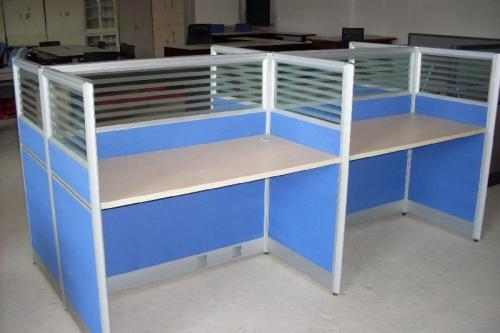
\includegraphics[width=0.62\textwidth]{assets/demo/photo-workbench-a.jpeg}
  \caption{公开内容生产场景的示意照片}
\end{figure}

\begin{figure}[H]
  \centering
  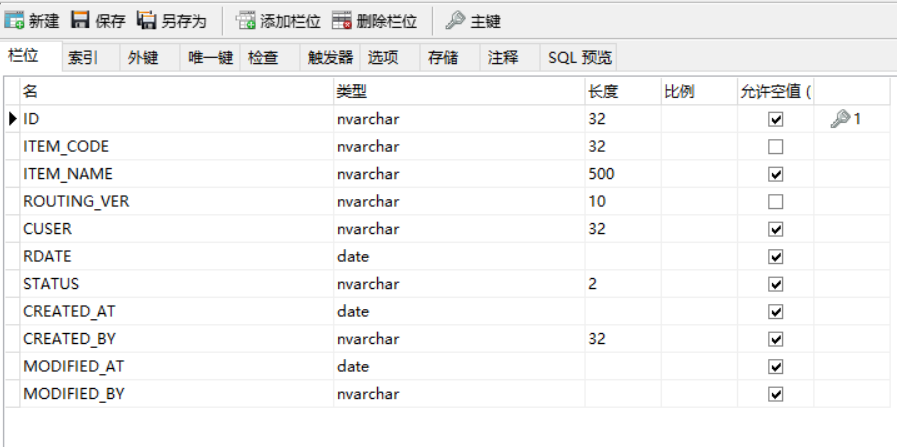
\includegraphics[width=0.76\textwidth]{assets/demo/screenshot-material-table.png}
  \caption{案例资料编码表的示意截图}
\end{figure}

\section{阶段特征对比表示例}

除了图像材料，毕业论文中还经常需要用表格把不同阶段的任务重点压缩成可比较的信息块。
表~\ref{tab:nju-stage-compare} 总结了本文对佐佐木希职业转型路径的示例性归纳，也展示了本模板中
宽表格的列宽控制和自动换行效果。

\begin{table}[H]
  \centering
  \caption{佐佐木希跨媒介职业转型阶段特征示例}
  \label{tab:nju-stage-compare}
  \begin{tabularx}{\textwidth}{>{\raggedright\arraybackslash}p{2.8cm}X}
    \toprule
    阶段 & 主要特征 \\
    \midrule
    模特起步期 & 依靠平面曝光建立初始识别度，形象标签相对集中，职业任务以高频出镜和风格固定化为主。 \\
    影视扩张期 & 通过电视剧、电影和综艺拓展受众面，开始从“单一外形资源”转向“角色与话题并行”的职业结构。 \\
    争议冲击期 & 私人事件引发叙事失控，外部评价高度集中，公共形象面临明显波动，传统媒体入口的缓冲能力下降。 \\
    平台重启期 & 借助社交平台与更生活化的内容重新建立更新节奏，把公众注意力从单次争议转回长期、稳定的日常表达。 \\
    \bottomrule
  \end{tabularx}
\end{table}

\section{小结}

从公开案例角度看，佐佐木希的职业转型说明了两个问题。第一，跨媒介转型并不只是“从 A 平台走向
B 平台”，而是伴随角色功能、更新节奏与叙事主导权的同步调整。第二，对模板项目而言，一篇公开、
可读、结构完整的示例论文，比空壳入口更能帮助用户理解如何替换自己的摘要、章节、图表和参考文献。
因此，`thesis-nju-master` 将 `main.tex` 恢复为默认正文入口，是更符合真实使用习惯的设计。
